\documentclass[12pt,a4paper]{amsart}
% ukazi za delo s slovenscino -- izberi kodiranje, ki ti ustreza
\usepackage[english]{babel}
\usepackage[utf8]{inputenc}
%\usepackage[T1]{fontenc}
\usepackage{amsmath,amssymb,amsfonts}
\usepackage{url}
%\usepackage[normalem]{ulem}
\usepackage[dvipsnames,usenames]{color}
\usepackage{caption}
\usepackage{lipsum}
\usepackage{tikz}
\usepackage{xcolor}
\usepackage[linesnumbered,ruled,vlined]{algorithm2e}
\usepackage{geometry}
\usepackage{array}


\usetikzlibrary{graphs}
\usetikzlibrary{graphs.standard}

\makeatletter
\renewcommand\section{\@startsection{section}{1}
  \z@{.5\linespacing\@plus.7\linespacing}{.5\linespacing}
  {\normalfont\scshape\large\centering}}
\renewcommand\subsection{\@startsection{subsection}{2}
  \z@{.5\linespacing\@plus.7\linespacing}{.5\linespacing}
  {\normalfont\scshape}}
\renewcommand\subsubsection{\@startsection{subsubsection}{3}
  \z@{.5\linespacing\@plus.7\linespacing}{-.5em}
  {\normalfont\itshape}}
\makeatother

% ne spreminjaj podatkov, ki vplivajo na obliko strani
\textwidth 15cm
\textheight 24cm
\oddsidemargin.5cm
\evensidemargin.5cm
\topmargin-5mm
\addtolength{\footskip}{10pt}
\pagestyle{plain}
\overfullrule=15pt % oznaci predlogo vrstico


% ukazi za matematicna okolja
\theoremstyle{definition} % tekst napisan pokoncno
\newtheorem{definicija}{Definition}[section]
\newtheorem{primer}[definicija]{Example}
\newtheorem{opomba}[definicija]{Remark}

\renewcommand\endprimer{\hfill$\diamondsuit$}

\theoremstyle{plain} % tekst napisan posevno
\newtheorem{lema}[definicija]{Lemma}
\newtheorem{izrek}[definicija]{Theorem}
\newtheorem{trditev}[definicija]{Statement}
\newtheorem{posledica}[definicija]{Corollary}
\newtheorem{conjecture}[definicija]{Conjecture}


% za stevilske mnozice uporabi naslednje simbole
\newcommand{\R}{\mathbb R}
\newcommand{\N}{\mathbb N}
\newcommand{\Z}{\mathbb Z}
\newcommand{\C}{\mathbb C}
\newcommand{\Q}{\mathbb Q}

% ukaz za slovarsko geslo
\newlength{\odstavek}
\setlength{\odstavek}{\parindent}
\newcommand{\geslo}[2]{\textbf{#1}\hspace*{3mm}\hangindent=\parindent\hangafter=1 #2}

% naslednje ukaze ustrezno popravi
\newcommand{\program}{Financial mathematics} % ime studijskega programa: Matematika/Finančna matematika
\newcommand{\imeavtorja}{Anej Rozman, Tanja Luštrek} % ime avtorja
\newcommand{\imementorja}{Assistant Professor Janoš Vidali} % akademski naziv in ime mentorja
\newcommand{\imesomentorja}{Professor Riste Škrekovski}
\newcommand{\naslovdela}{Rich-Neighbor Edge Colorings}
\newcommand{\letnica}{2023} %letnica diplome

\begin{document}

\thispagestyle{empty}
{\large
\noindent UNIVERSITY OF LJUBLJANA\\[1mm]
FACULTY OF MATHEMATICS AND PHYSICS\\[5mm]
\program\ -- 1st cycle}
\vfill

\begin{center}{\large
\imeavtorja\\[2mm]
{\bf \naslovdela}\\[10mm]
Term Paper in Finance Lab\\[2mm]
Long Presentation\\[1cm]
Advisers: \imementorja, \\ \imesomentorja\\[2mm]}
\end{center}
\vfill

{\large
Ljubljana, \letnica}
\pagebreak

\thispagestyle{empty}
\tableofcontents
\pagebreak

\section{Introduction}

    In this paper we set out to analyse an open conjecture in a modern graph theory problem known as rich-neighbor edge coloring.

    \begin{definicija}
        In an edge coloring, an edge $e$ is called $rich$ if all edges adjacent to $e$ have different colors. An edge coloring is 
        called a $rich\text{-}neighbor \ edge \ coloring$ if every edge is adjacent to some rich edge.
    \end{definicija}

    \begin{definicija}
        $X'_{rn}(G)$ denotes the smallest number of colors for which there exists a rich-neighbor edge coloring.
    \end{definicija}

    \begin{conjecture}
        For every graph $G$ of maximum degree $\Delta$, $X'_{rn}(G) \leq 2\Delta - 1$ holds.
    \end{conjecture}

    \begin{primer}
    Let's take a look at the Petersen graph and an example of a rich-neighbor edge coloring.\\
    \begin{center}
        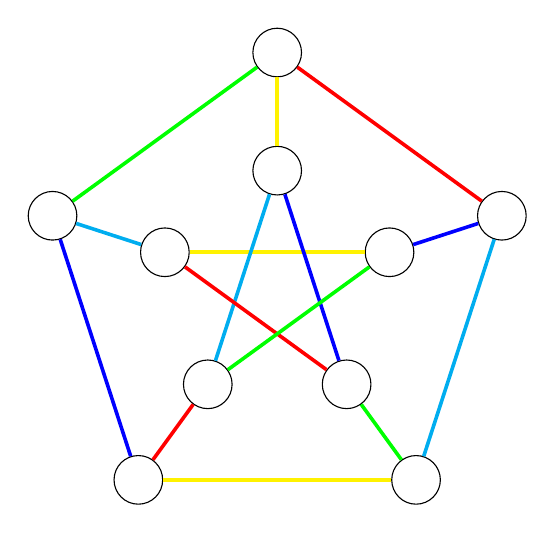
\begin{tikzpicture}[every node/.style={draw,circle, style={text opacity=0}}]
            \graph[clockwise, radius=3cm] {subgraph C_n [n=5,name=A] };
            \graph[clockwise, radius=1.5cm] {subgraph I_n [n=5,name=B] };

            % Define edge colors for the graph
            \draw[yellow, line width=1.3pt] (A 1) -- (B 1);
            \draw[blue, line width=1.3pt] (A 2) -- (B 2);
            \draw[green, line width=1.3pt] (A 3) -- (B 3);
            \draw[red, line width=1.3pt] (A 4) -- (B 4);
            \draw[cyan, line width=1.3pt] (A 5) -- (B 5);
            \draw[red, line width=1.3pt] (A 1) -- (A 2);
            \draw[cyan, line width=1.3pt] (A 2) -- (A 3);
            \draw[yellow, line width=1.3pt] (A 3) -- (A 4);
            \draw[blue, line width=1.3pt] (A 4) -- (A 5);
            \draw[green, line width=1.3pt] (A 5) -- (A 1);
            \draw[yellow, line width=1.3pt] (B 5) -- (B 2);
            \draw[cyan, line width=1.3pt] (B 4) -- (B 1);
            \draw[blue, line width=1.3pt] (B 3) -- (B 1);
            \draw[red, line width=1.3pt] (B 5) -- (B 3);
            \draw[green, line width=1.3pt] (B 4) -- (B 2);
        \end{tikzpicture}\\
    \end{center}
    We can see that for the Petersen graph (which is 3-regular) we can find an appropriate coloring with 5 colors so $X'_{rn} \leq 5 \leq 2 \cdot 3 - 1 = 5$. This shows that the conjecture holds for this graph.
    \end{primer}\\
    \textcolor{white}{i\\ i\\ i\\ i\\ i\\ i\\ i\\ i\\ i\\ i\\ i\\ i\\ i\\ i\\}
    \pagebreak


\section{Algorithms}
    \subsection{Integer Programming}

        Using SageMath we constructed an integer programming model that finds a rich-neighbor edge coloring for a given graph using the smallest number of colors possible. Our interger program looks like this:\\

        minimize $t$ \hfill \footnotesize{\textcolor{black}{we minimize the number of colors we need}}\\
        %vsoto sm dala do 2delta - 1 prej je bla do k a je to kul???
        subject to $\forall e: \quad \sum_{i=1}^{2\Delta - 1} x_{ei} = 1$ \hfill \footnotesize{\textcolor{black}{each edge is exactly one color}}\\

        \ \ \ \ \ \ \ \ \ \ \ \ \ \ $\forall i \ \forall u \ \forall v, w \sim u, v \neq u: \quad x_{uv, i} + x_{uw, i} \leq 1$\\[0.1mm]
        \textcolor{white}{hihi} \hfill \footnotesize{\textcolor{black}{edges with the same vertex are a different color}}\\

        \ \ \ \ \ \ \ \ \ \ \ \ \ \ $\forall e \ \forall i: \quad x_{ei} \cdot i \leq t$ \hfill \footnotesize{\textcolor{black}{we use less or equal to $t$ colors}}\\

        \ \ \ \ \ \ \ \ \ \ \ \ \ \ $\forall i \ \forall uv \ \forall w \sim u, w \neq v \ \forall z \sim v, z \neq u, w: \quad x_{uw, i} + x_{vz, i} + y_{uv} \leq 2$ \hfill \\[0.1mm]
        \textcolor{white}{hihi} \hfill \footnotesize{\textcolor{black}{$uv$ is a rich edge $\Leftrightarrow$ all adjacent edges are a different color}}\\

        \ \ \ \ \ \ \ \ \ \ \ \ \ \ $\forall e: \quad \sum_{f \sim e}y_f \geq 1$ \hfill \footnotesize{\textcolor{black}{every edge is adjacent to some rich edge}}\\

        %\ \ \ \ \ \ \ \ \ \ \ \ \ \ $t \geq 2 \Delta - 1$ \hfill \footnotesize{\textcolor{black}{we use $\geq 2 \Delta - 1$ colors}}\\

        \ \ \ \ \ \ \ \ \ \ \ \ \ \ $\forall e: \quad 0 \leq y_{e} \leq 1$, $y_{e} \in \Z$\\

        \ \ \ \ \ \ \ \ \ \ \ \ \ \ $\forall e \ \forall i: \quad 0 \leq x_{ei} \leq 1$, $x_{ei} \in \Z$,\\

        where
        \begin{align*}        x_{ei} = \begin{cases}
                    1, \  \text{if edge $e$ has color $i$} \\
                    0, \  \text{otherwise}
            \end{cases} & \text{and} & 
            y_{e} = \begin{cases}
                1, \  \text{if edge $e$ is rich} \\
                0, \  \text{otherwise.}
            \end{cases}
        \end{align*}\\


        %js bi rekla da ne fiksiramo st barv in vsaka povezava ma 2delta -2 sosednjih povezav, ampak sklep pa drzi kr pac se to povezavo stejemo da more bit svoje barve
        In our implementation of the ILP we fix the number of colors to $2 \Delta - 1$ by adding the following constraint
        $$
            t = 2\Delta - 1,
        $$
        since the coloring can't be made with less colors (every edge has $2 \Delta - 2$ neighboring edges and the edge itself has to be a different color) and any more colors do not satisfie the conjecture. Therefore we only check if the program has a solution that satisfies all the constraints and the conjecture. In theory this doesn't make the program faster, but in our practice tests it did make a significant differnece.\\

        Our implementation of the IPL is demonstrated in the following code.
        \begin{algorithm}[!htbp]
            \caption{richNeighbor}\label{algo:richNeighbor}
            \LinesNumberedHidden
            \DontPrintSemicolon
            \SetAlgoNlRelativeSize{0}
            \SetAlgoNlRelativeSize{-1}
            \SetAlgoNlRelativeSize{1}
            \SetKwInput{KwInput}{Input}
            \SetKwInput{KwOutput}{Output}

            \SetKwFunction{FMain}{richNeighbor}

            \KwInput{Graph $G$}
            \KwOutput{Colors $colors$, Rich edges $richEdges$}

            $p \gets$ MixedIntegerLinearProgram(maximization = False)\;
            $x \gets p.new\_variable(binary = True)$\;
            $y \gets p.new\_variable(binary = True)$\;
            $t \gets p.new\_variable(integer = True)$\;
            $p.set\_objective(t[0])$\;

            $\text{maxCol} \gets 2 \cdot G.degree()[0] - 1$\;

            $p.add\_constraint(t[0] = \text{maxCol})$\;

            \For{$e$ in $G.edges(\text{labels} = \text{False})$}{
                $p.add\_constraint(\sum_{i=1}^{\text{maxCol}} x[\text{Set}(e), i] = 1)$\;
            }

            \For{$(u,v)$ in $G.edges(\text{labels} = \text{False})$}{
                $p.add\_constraint(\sum_{j \in G[u]} y[\text{Set}((u, j))] + \sum_{l \in G[v]} y[\text{Set}((l, v))] - 2y[\text{Set}((u, v))] \geq 1)$\;
            }

            \For{$e$ in $G.edges(\text{labels} = \text{False})$}{
                \For{$i$ in $1$ to $\text{maxCol}$}{
                    $p.add\_constraint(i \cdot x[\text{Set}(e), i] \leq t[0])$\;
                }
            }

            \For{$i$ in $1$ to $\text{maxCol}$}{
                \For{$(u,v)$ in $G.edges(\text{labels} = \text{False})$}{
                    \For{$w$ in $G[u]$}{
                        \If{$w = v$}{
                            \textbf{continue}\;
                        }
                        $p.add\_constraint(x[\text{Set}((u, v)), i] + x[\text{Set}((u, w)), i] \leq 1)$\;
                    }
                    \For{$z$ in $G[v]$}{
                        \If{$z = u$}{
                            \textbf{continue}\;
                        }
                        $p.add\_constraint(x[\text{Set}((u, v)), i] + x[\text{Set}((v, z)), i] \leq 1)$\;
                    }
                }
            }

            \For{$(u, v)$ in $G.edges(\text{labels}=False)$}{
                \For{$w$ in $G.neighbors(u)$}{
                    \For{$z$ in $G.neighbors(v)$}{
                        \If{$w = v$ or $z = u$}{
                            \textbf{continue}\;
                        }
                        \For{$i$ in $1$ to $\text{maxCol}$}{
                            $p.add\_constraint(x[\text{Set}((u, w)), i] + x[\text{Set}((v, z)), i] + y[\text{Set}((u, v))] \leq 2)$\;
                        }
                    }
                }
            }

            %\Try{
            %    $p.solve()$\;
            %    $colors \gets p.get\_values(x)$\;
            %    $richEdges \gets p.get\_values(y)$\;
            %}
            %\Catch{ValueError}{
            %    $\text{print}(\text{f'BINGO! The graph }{G}\text{ doesn't have a rich-neighbor edge coloring! \n' + f'Edges: }{G.edges()} \text{; \n' + f'Adjacency matrix: }{G.adjacency\_matrix()} \text{; \n' + f'Neighbors: }{G.neighbors()})$\;
            %    \Return \text{False, False}\;
            %}
            %
            \Return $colors$, $richEdges$\;
            \end{algorithm}

\pagebreak
    \subsection{Iterative Algorithm}
            
            We also implemented an iterative algorithm that finds a rich-neighbor edge coloring for a given graph. The algorithm works by assigning a color to an edge and then checking if the coloring is valid. If it is, we move on to the next edge, otherwise we try a different color. If we can't find a valid coloring with $2 \Delta - 1$ colors, we increase the number of colors by one and try again.\\
    
            The algorithm is not guaranteed to find a coloring with $2 \Delta - 1$ colors, but it is guaranteed to find a coloring with $2 \Delta$ colors.\\
    
            The algorithm is very fast for footnotesize graphs, but it becomes too slow for graphs with more than 10 vertices. Ta tekst so smeti ma tle bi pc mogli mal blefirat da je iterativn algoritm pocasnejsi od ILPja.\\

\section{Complete search}

    As illustrated in Table \ref{table:1}, the number of $k$-regular graphs on $n$ vertices is of exponential growth. This poses a computational challenge, as exhaustively examining all such graphs becomes impractical for larger values of $n$. The sheer scale of potential combinations makes a complete search unfeasible within reasonable timeframes.

    However, a thorough exploration of all $k$-regular graphs remains viable and efficient for footnotesize values of $n$.

    \begin{table}[!htbp]
        \centering
        \begin{tabular}{|c|c|c|c|c|}
            \hline
            Vertices & Degree 4 & Degree 5 & Degree 6 & Degree 7 \\
            \hline
            5 & 1 & 0 & 0 & 0 \\
            6 & 1 & 1 & 0 & 0 \\
            7 & 2 & 0 & 1 & 0 \\
            8 & 6 & 3 & 1 & 1 \\
            9 & 16 & 0 & 4 & 0 \\
            10 & 59 & 60 & 21 & 5 \\
            11 & 265 & 0 & 266 & 0 \\
            12 & 1544 & 7848 & 7849 & 1547 \\
            13 & 10778 & 0 & 367860 & 0 \\
            14 & 88168 & 3459383 & 21609300 & 21609301 \\
            15 & 805491 & 0 & 1470293675 & 0 \\
            16 & 8037418 & 2585136675 & 113314233808 & 733351105934 \\
            \hline
        \end{tabular}
        \caption{Number of $k$-regular graphs on $n$ vertices}
        \label{table:1}
    \end{table}

    \subsection{Graph generation}
        Graphs for the complete search were taken from a collection of \texttt{.tex} files, provided by Professor Skrekovski. The files contain all $k$-regular graphs on $n$ vertices up to 15 vertices.

\section{Random Search}

    In addition to examining the hypothesis for smaller graphs, we were also interested in checking if the conjecture holds for larger graphs. The challenge is, as said before, the pure impracticality of systematically testing all potential scenarios of colorings in graphs with many vertices.

    Recognizing the enormity of this task, a random search algoritm seemed a natural continuation of our problem. Here we opted for a modification approach.\\

    We start with a random graph, check if the conjecture holds and then 
    modify it in a way that preserves the regularity and connectedness. We repeat this process indefinetly. Since, if a rich-neighbor edge coloring exists in a given graph there is a bigger probability that it also exists in similar graphs, therefore, on every iteration, there is a footnotesize probability that we generate a completely new random graph and start again.  

    %Razlog je, da ce je v grafu obstaja rich neighbor edge coloring potem je vecja verjetnost da bo v bliznjih grafih prav tako obstajala, zato dopuscamo manjso moznost da popolnoma na novo generiramo graf.

    Written below is the algorithm for modifying graphs. First it selects two random edges and deletes them. Then it assigns a random probability to $p$ and based on the value of $p$ it adds back to different edges we did not have before. It repeats this until it gets a connected modified graph.
    \begin{algorithm}[!htbp]
        \caption{tweak}\label{algo:tweakGraph}
        \LinesNumberedHidden
        \DontPrintSemicolon
        \SetAlgoNlRelativeSize{0}
        \SetAlgoNlRelativeSize{-1}
        \SetAlgoNlRelativeSize{1}
        \SetKwInput{KwInput}{Input}
        \SetKwInput{KwOutput}{Output}
        
        \SetKwFunction{FTweakGraph}{tweakGraph}
        
        \KwInput{Graph $G$}
        \KwOutput{Tweaked graph $T$}
        

            $T \gets \text{graph.copy()}$\;
            
            $e_1 \gets T.\text{random\_edge()}$\;
            $u_1, v_1, \text{extra}_1 \gets e_1$\;
            $T.\text{delete\_edge}(e_1)$\;
            
            $e_2 \gets T.\text{random\_edge()}$\;
            $u_2, v_2, \text{extra}_2 \gets e_2$\;
            $T.\text{delete\_edge}(e_2)$\;
        
            $p \gets \text{random}()$\;
            \If{$p < 0.5$}{
                $T.\text{add\_edge}(u_1, u_2)$\;
                $T.\text{add\_edge}(v_1, v_2)$\;
            }\Else{
                $T.\text{add\_edge}(u_1, v_2)$\;
                $T.\text{add\_edge}(v_1, u_2)$\;
            }
            
            \If{not $T.\text{is\_connected}()$}{
                \Return \text{tweakGraph}(\text{graph})\;
            }
            
            \Return $T$\;
        
        
        \end{algorithm}

    
    \pagebreak
    \subsection{Graph generation}
        Since we only need one graph to start our iterative process, we can generate it randomly using the built in sage function \texttt{graphs.RandomRegular}.

\section{Checking the coloring} %tukej daj algoritma chack coloring in check richness. Ostalo bom js napisu
    dodaj še opisa algoritmov
    \begin{algorithm}[!htbp]
        \caption{Check Coloring}\label{algo:checkColoring}
        \LinesNumberedHidden
        \DontPrintSemicolon
        \SetAlgoNlRelativeSize{0}
        \SetAlgoNlRelativeSize{-1}
        \SetAlgoNlRelativeSize{1}
        \SetKwInput{KwInput}{Input}
        \SetKwInput{KwOutput}{Output}

        \SetKwFunction{FCheckColoring}{checkColoring}

        \KwInput{Graph $G$, Coloring $coloring$}
        \KwOutput{Boolean indicating proper coloring}

        \For{$v$ in $G.vertices()$}{
            $col \gets \text{set()}$\;
            \For{$w$ in $G.neighbors(v)$}{
                \For{$i$ in $range(1, 2 \cdot G.degree()[0])$}{
                    \If{$coloring[(\text{Set}((v, w)), i)] = 1$}{
                        $col.\text{add}(i)$\;
                    }
                }
            }
            \If{$\text{len}(col) \neq \text{len}(G.neighbors(v))$}{
                \Return \text{False}\;
            }
        }
        \Return \text{True}\;
    \end{algorithm}


    \begin{algorithm}[!htbp]
        \caption{Check Richness}\label{algo:checkRichness}
        \LinesNumberedHidden
        \DontPrintSemicolon
        \SetAlgoNlRelativeSize{0}
        \SetAlgoNlRelativeSize{-1}
        \SetAlgoNlRelativeSize{1}
        \SetKwInput{KwInput}{Input}
        \SetKwInput{KwOutput}{Output}
        
        \SetKwFunction{FCheckRichness}{checkRichness}
        
        \KwInput{Graph $G$, Rich edges $richEdges$}
        \KwOutput{Boolean indicating proper rich-neighbor edge coloring}
        
        \For{$(u, v)$ in $G.edges(labels = False)$}{
            $S \gets 0$\;
            \For{$w$ in $G.neighbors(u)$}{
                \If{$w = v$}{
                    $S \gets S + richEdges[\text{Set}((u, w))]$\;
                }
            }
            \For{$z$ in $G.neighbors(v)$}{
                \If{$z = u$}{
                    $S \gets S + richEdges[\text{Set}((v, z))]$\;
                }
            }
            \If{$S = 0$}{
                \Return \text{False}\;
            }
        }
        \Return \text{True}\;
    \end{algorithm}
    
    
    \pagebreak


\section{Findings}

\section{Conclusion}



\end{document}